%Notes by Harsh Mistry 
%CS 350
%Based on Template From  https://www.cs.cmu.edu/~ggordon/10725-F12/template.tex

\documentclass[twoside]{article}
\setlength{\oddsidemargin}{0.25 in}
\setlength{\evensidemargin}{-0.25 in}
\setlength{\topmargin}{-0.6 in}
\setlength{\textwidth}{6.5 in}
\setlength{\textheight}{8.5 in}
\setlength{\headsep}{0.75 in}
\setlength{\parindent}{0 in}
\setlength{\parskip}{0.1 in}
\usepackage{amsfonts,graphicx, amssymb}
\usepackage[fleqn]{amsmath}
\usepackage{fixltx2e}
\usepackage{color}
\usepackage{tcolorbox}
\usepackage{lipsum}
\usepackage{listings}
\usepackage{scrextend}
\tcbuselibrary{skins,breakable}
\usetikzlibrary{shadings,shadows}
\newcounter{lecnum}
\renewcommand{\thepage}{\thelecnum-\arabic{page}}
\renewcommand{\thesection}{\thelecnum.\arabic{section}}
\renewcommand{\theequation}{\thelecnum.\arabic{equation}}
\renewcommand{\thefigure}{\thelecnum.\arabic{figure}}
\renewcommand{\thetable}{\thelecnum.\arabic{table}}
\newcommand{\lecture}[4]{
   \pagestyle{myheadings}
   \thispagestyle{plain}
   \newpage
   \setcounter{lecnum}{#1}
   \setcounter{page}{1}
   
   \graphicspath{ {images/} }
   
%Info Box 
   \begin{center}
   \framebox{
      \vbox{\vspace{2mm}
    \hbox to 6.28in { {\bf CS 350 - Operating Systems
	\hfill Winter 2018} }
       \vspace{4mm}
       \hbox to 6.28in { {\Large \hfill Lecture #1: #2  \hfill} }
       \vspace{2mm}
       \hbox to 6.28in { {\it Lecturer: #3 \hfill Notes By: #4} }
      \vspace{2mm}}
   }
   \end{center}
   
   \markboth{Lecture #1: #2}{Lecture #1: #2}



 
}

\renewcommand{\cite}[1]{[#1]}
\def\beginrefs{\begin{list}%
        {[\arabic{equation}]}{\usecounter{equation}
         \setlength{\leftmargin}{2.0truecm}\setlength{\labelsep}{0.4truecm}%
         \setlength{\labelwidth}{1.6truecm}}}
\def\endrefs{\end{list}}
\def\bibentry#1{\item[\hbox{[#1]}]}

\newcommand{\fig}[3]{
			\vspace{#2}
			\begin{center}
			Figure \thelecnum.#1:~#3
			\end{center}
	}

\newtheorem{theorem}{Theorem}[lecnum]
\newtheorem{lemma}[theorem]{Lemma}
\newtheorem{ex}[theorem]{Example}
\newtheorem{proposition}[theorem]{Proposition}
\newtheorem{claim}[theorem]{Claim}
\newtheorem{corollary}[theorem]{Corollary}
\newtheorem{definition}[theorem]{Definition}
\newenvironment{proof}{{\bf Proof:}}{\hfill\rule{2mm}{2mm}}
\newcommand\E{\mathbb{E}}




%color definitions :
\definecolor{darkred}{rgb}{0.55, 0.0, 0.0}
\definecolor{lightcoral}{rgb}{0.94, 0.5, 0.5}
\definecolor{tomato}{rgb}{1.0, 0.39, 0.28}
\definecolor{lightgray}{rgb}{.9,.9,.9}
\definecolor{darkgray}{rgb}{.4,.4,.4}
\definecolor{purple}{rgb}{0.65, 0.12, 0.82}
\definecolor{lightgreen}{rgb}{0.56, 0.93, 0.56}
\definecolor{darkgreen}{rgb}{0.0, 0.2, 0.13}
\definecolor{limegreen}{rgb}{0.2, 0.8, 0.2}
\definecolor{lightblue}{rgb}{0.68, 0.85, 0.9}
\definecolor{darkblue}{rgb}{0.0, 0.0, 0.55}


%Environments
\newenvironment{exblock}[1]{%
    \tcolorbox[beamer,%
    noparskip,breakable,
    colback=lightgreen,colframe=darkgreen,%
    colbacklower=limegreen!75!lightgreen,%
    title=#1]}%
    {\endtcolorbox}

\newenvironment{ablock}[1]{%
    \tcolorbox[beamer,%
    noparskip,breakable,
    colback=lightcoral,colframe=darkred,%
    colbacklower=tomato!75!lightcoral,%
    title=#1]}%
    {\endtcolorbox}

\newenvironment{cblock}[1]{%
    \tcolorbox[beamer,%
    noparskip,breakable,
    colback=lightblue,colframe=darkblue,%
    colbacklower=darkblue!75!lightblue,%
    title=#1]}%
    {\endtcolorbox}


%Languages
\lstdefinelanguage{JavaScript}{
  keywords={typeof, new, true, false, catch, function, return, null, catch, switch, var, if, in,  fi, while, do, else, case, break, const},
  keywordstyle=\color{blue}\bfseries,
  ndkeywords={class, export, boolean, throw, implements, import, this, struct},
  ndkeywordstyle=\color{darkgray}\bfseries,
  identifierstyle=\color{black},
  sensitive=false,
  comment=[l]{//},
  morecomment=[s]{/*}{*/},
  commentstyle=\color{purple}\ttfamily,
  stringstyle=\color{red}\ttfamily,
  morestring=[b]',
  morestring=[b]"
}

%Listings
\lstset{
   language=JavaScript,
   backgroundcolor=\color{lightgray},
   extendedchars=true,
   basicstyle=\footnotesize\ttfamily,
   showstringspaces=false,
   showspaces=false,
   numbers=left,
   numberstyle=\footnotesize,
   numbersep=9pt,
   tabsize=2,
   breaklines=true,
   showtabs=false,
   captionpos=b
}






%Start of Document 
\begin{document}

\lecture{5}{January 17, 2018}{Lesley Istead}{Harsh Mistry}

\section{Synchronization Continued}


\subsection{Spin Locks in OS/161}
\begin{center}
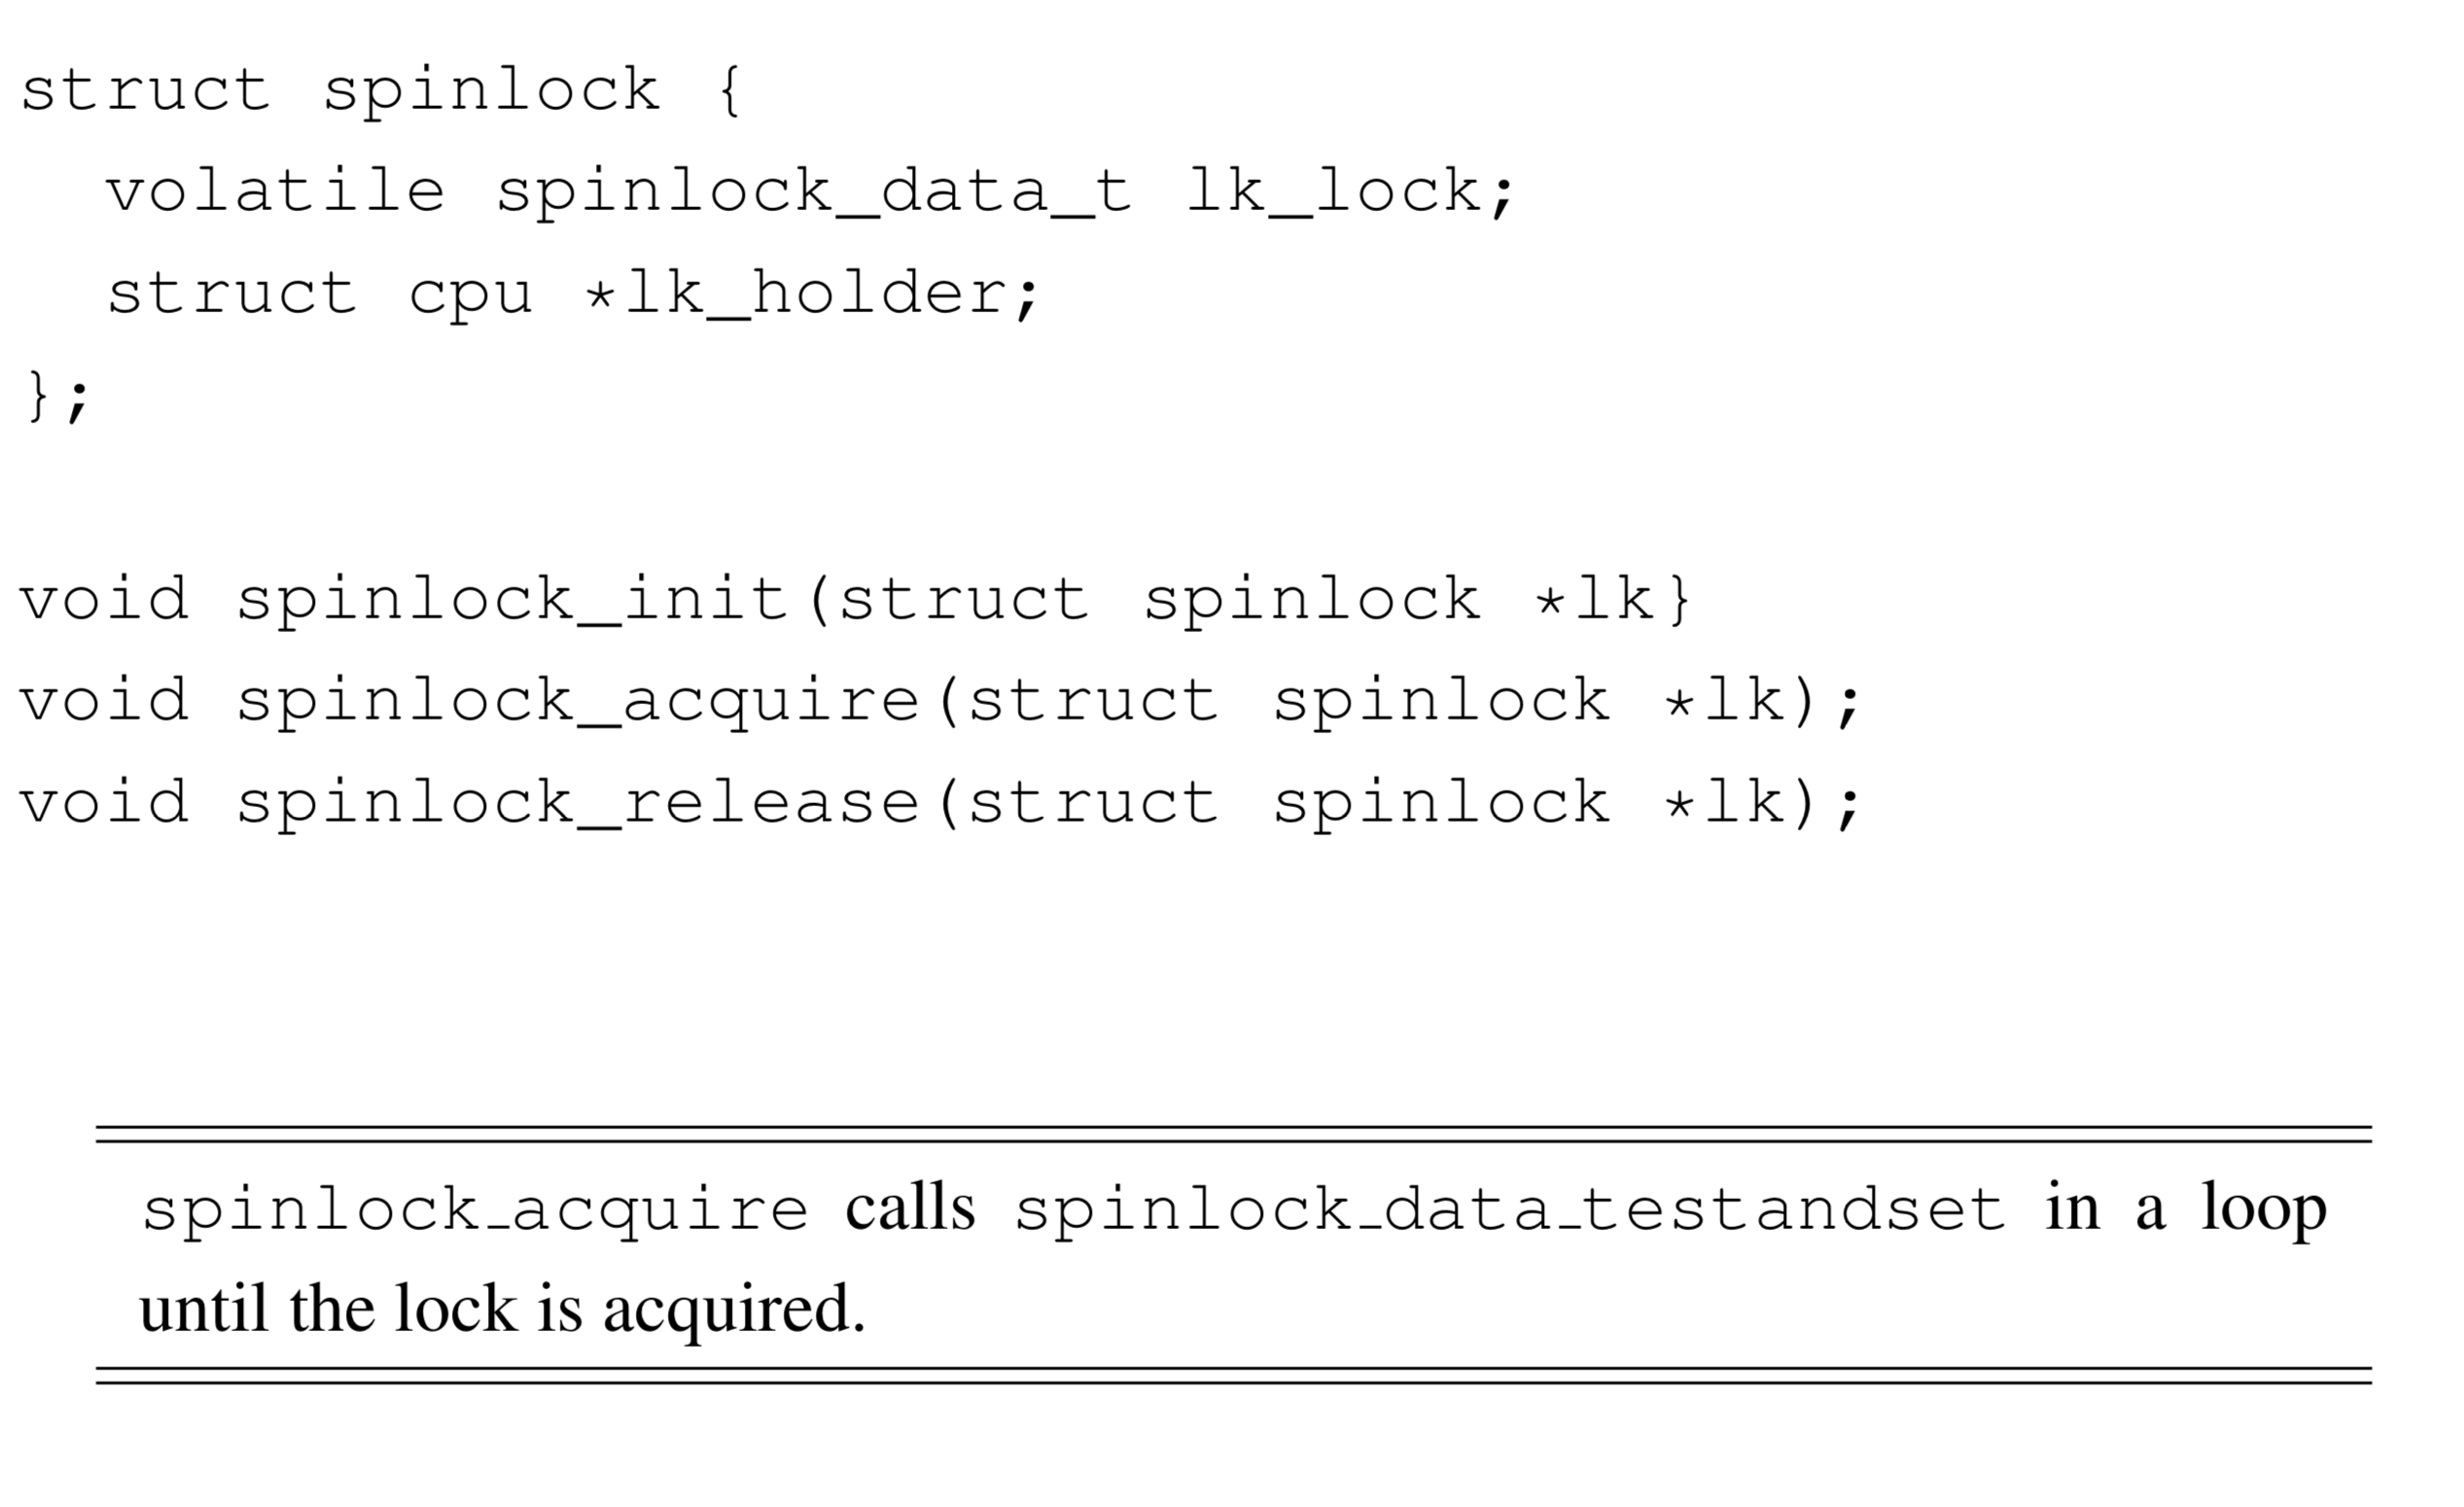
\includegraphics[scale=0.2]{5}
\end{center}

\begin{ex} Spin-lock implementation for MIPS using in line assembly 
\begin{center}
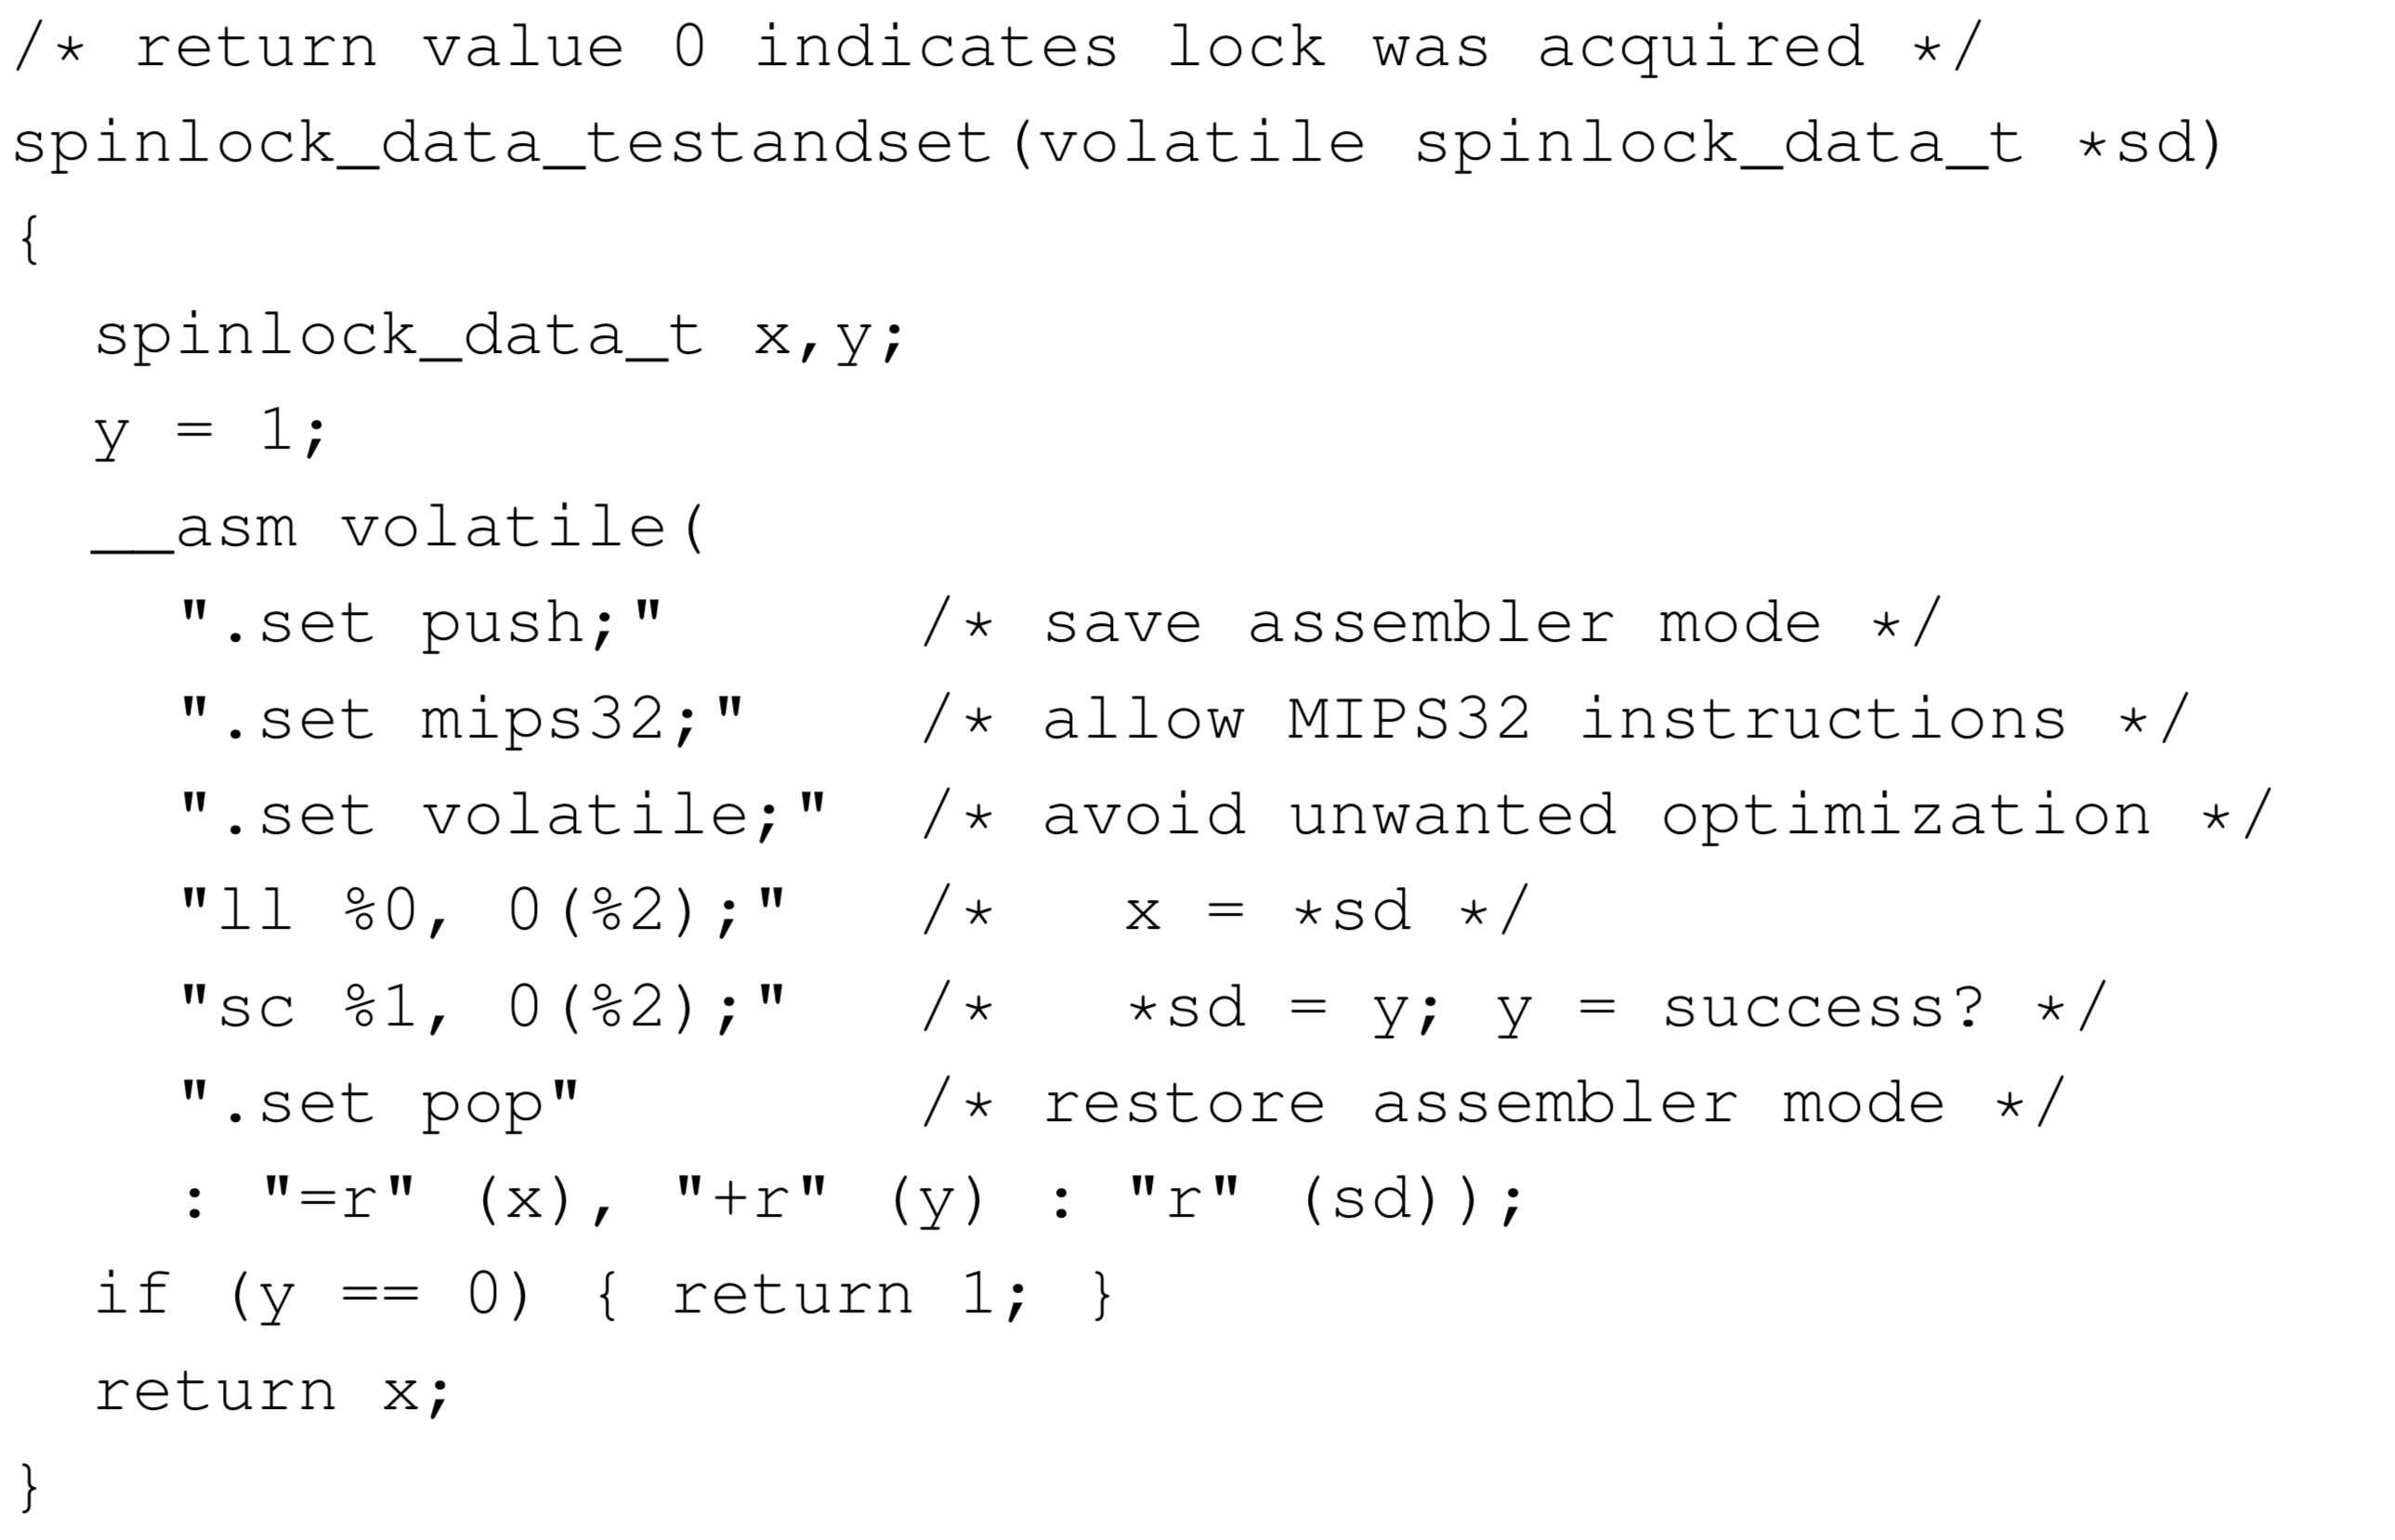
\includegraphics[scale=0.2]{6}
\end{center}
\end{ex}

\subsection{Thread Blocking}
\begin{itemize}
\item Sometimes a thread will wait for something e.g
\begin{itemize}
\item wait for lock to be released
\item wait for data from a (relatively) slow device
\item wait for input from a keyboard
\item wait for busy device to become idle
\end{itemize}
\item When a thread blocks, its stops running:
\begin{itemize}
\item the scheduler chooses a new thread to run 
\item a context switch from teh blocking thread to the new thread occurs
\item the blocking thread is queued in a \verb|wait queue| (not on the ready list)
\item Eventually, a blocked thread is signalled and awakened by another thread
\end{itemize}
\end{itemize}

\subsection{Wait Channels in OS/161}
\begin{itemize}
\item  Wait channels are used to implement thread blocking in OS/161
\begin{itemize}
\item \verb|void wchan_sleep(struct whan *wc);|, blocks calling a thread on wait channel and causes a context switch 
\item \verb|void wchan_wakeall(struct wchan *wc);|, unblock all threads sleeping on wait channel \verb|wc|
\item \verb|void wchan_wakeone(struct wchan *wc);|, unblock one thread sleeping on wait channel \verb|wc|
\item \verb|void wchan_lock(struct wchan *wc);|, prevents operations on wait channel \verb|wc|
\end{itemize}
\item There can also be many different wait channels, holding thread that are blocked for different reasons. 
\end{itemize}

\subsection{OS/161 Lock Implementation}
\begin{center}
\textbf{\textcolor{red}{Pseudo Code For A1 Q1}}
\end{center}
\textbf{Acquire :}
\begin{lstlisting}
spin_acquire (lock->spin) 
KASSERT(!lockowner)
KASSERT(!lock == null) 
while (lock->held) {
	wchan_lock(lock->wc);
	spin_release(lock->wc);
	wchan_sleep(lock->wc);
	spin_aquire(lock->spin)
}
lock->held = 1;
lock->owner - curthread;
spin_release(lock->spin);
\end{lstlisting}
\textbf{Release :}
\begin{lstlisting}
KASSERT(Owns the block) 
spin_acquire(lock->spin);
lock->held = 0;
lock->owner = null;
wchan_wakeone(lock->wc);
spin_release(lock->spin)
\end{lstlisting}


\end{document}


